\subsection{Company growth}

\begin{frame}{Bob's company is being very successfull...}
  \begin{center}
    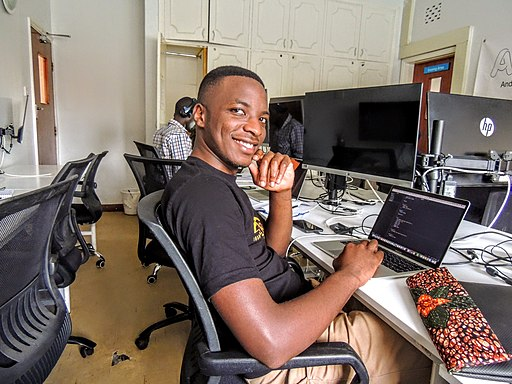
\includegraphics[width=.7\textwidth]{./assets/bob.jpeg}
  \end{center}
\end{frame}

\begin{frame}{A company growth... so its architecture}
  \begin{center}
    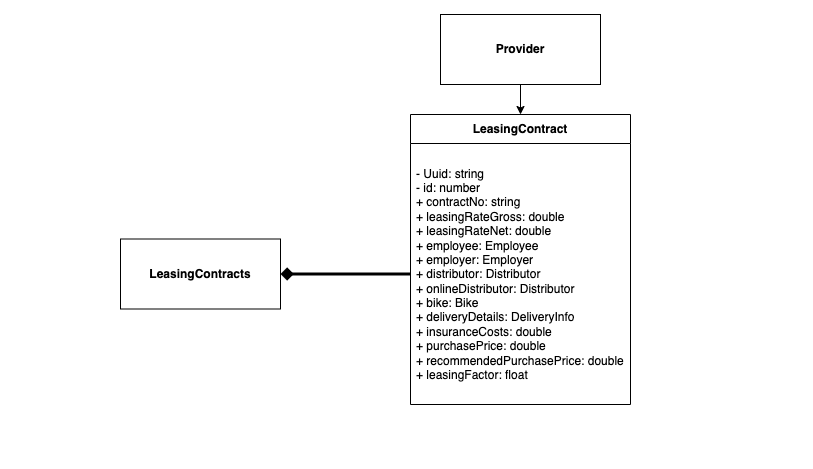
\includegraphics[scale=.5]{./assets/model1}
  \end{center}
\end{frame}

\begin{frame}{A company growth... so its architecture}
  \begin{center}
    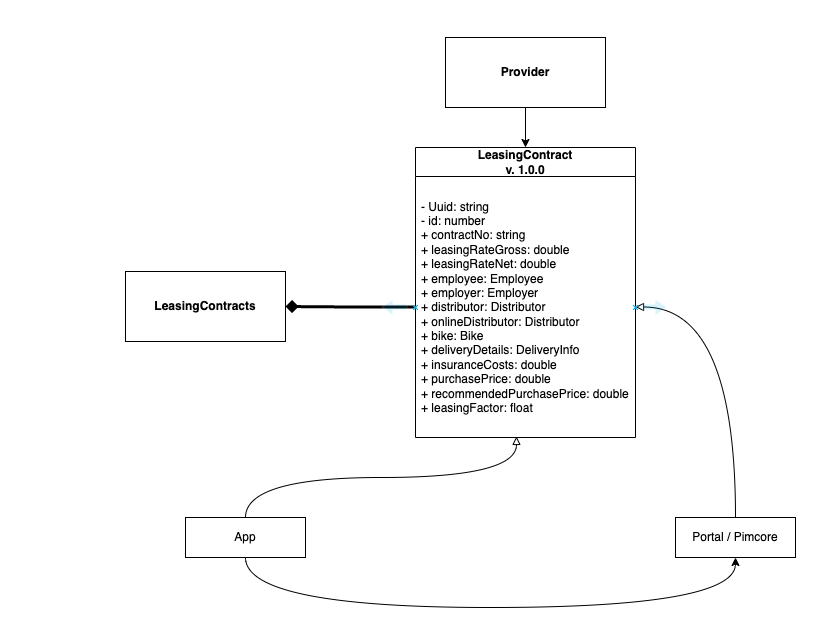
\includegraphics[scale=.35]{./assets/model2}
  \end{center}
\end{frame}


\begin{frame}{A company growth... so its architecture}
  \begin{center}
    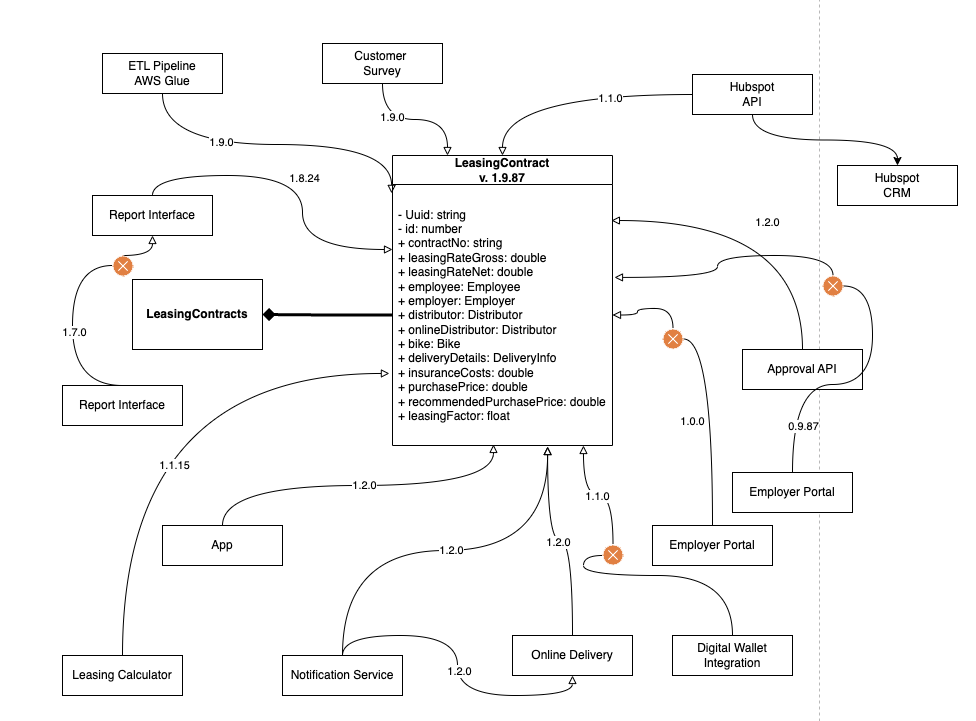
\includegraphics[scale=.3]{./assets/model3}
  \end{center}
\end{frame}


\begin{frame}{Bob is happy...}
  \begin{center}
    
\includegraphics[scale=.45]{./assets/chaos}
  \end{center}
\end{frame}

\begin{frame}{The Problem...}
  \begin{shadequote}
    \hspace{1cm} Every time we touch one service, all the others break :(
  \end{shadequote}
  \begin{columns}
    \begin{column}{0.6\textwidth}
      \begin{itemize}
        \item Dependency hell
        \item Devs don't have confidence in deploying changes
        \begin{itemize}
          \item Consequences of changes are hard to track
          \item Distributed architectures are hard to test
        \end{itemize}
      \end{itemize}
    \end{column}
    \begin{column}{0.4\textwidth}
      
\includegraphics[scale=.3]{./assets/sad_dev.jpeg}
    \end{column}
  \end{columns}
  \end{frame}

\begin{frame}{Architecture example: Online Delivery}
  \begin{center}
    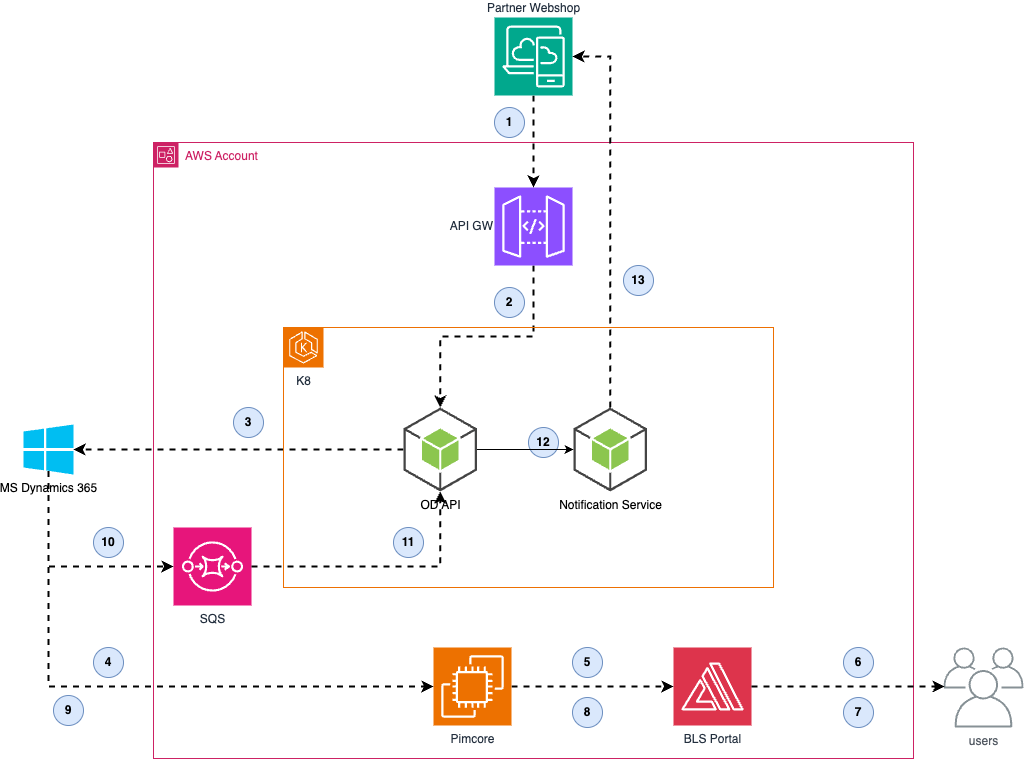
\includegraphics[scale=.3]{./assets/od.png}
  \end{center}
\end{frame}

\begin{frame}{Architecture example: Leasing Calculator}
  \begin{center}
    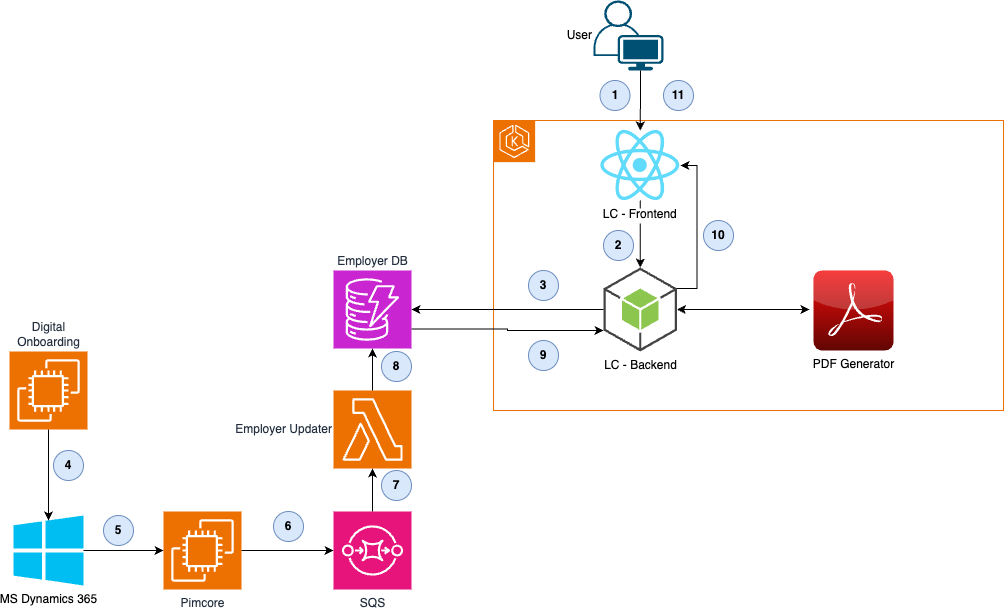
\includegraphics[scale=.3]{./assets/lc.png}
  \end{center}
\end{frame}

\begin{frame}[fragile]{Updating a microservice: the sad Atlassian case}

  \begin{columns}
    \begin{column}{0.5\textwidth}
      \begin{lstlisting}[language=json]
{
  "users": "Mike",
  "address": "Something"
}
      \end{lstlisting}
    \end{column}
    \begin{column}{0.5\textwidth}
        \begin{lstlisting}[language=json]
{
  "user": "Mike",
  "address": "Something"
}
        \end{lstlisting}
    \end{column}
  \end{columns}
\begin{center}
  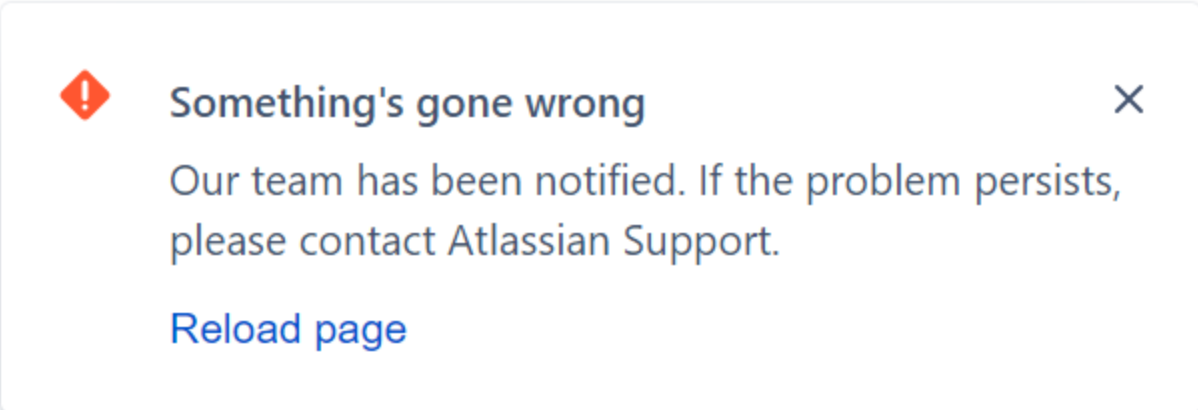
\includegraphics[scale=.4]{./assets/atlassian}
\end{center}
\end{frame}

\subsection{Test Typology}

\begin{frame}{Test Typology}
  \begin{center}
    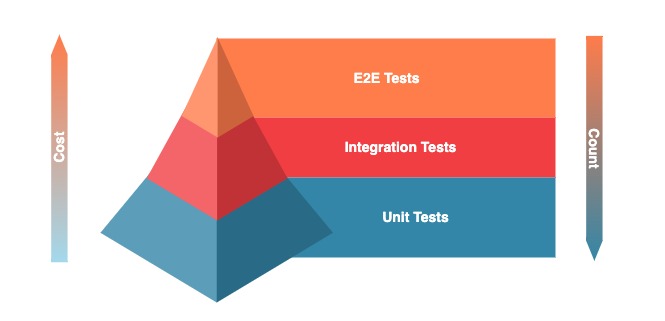
\includegraphics[scale=.6]{./assets/test_pyramid}
  \end{center}
\end{frame}

\begin{frame}{The problem with Unit Tests alone}
  \begin{itemize}
    \item Local changes, even if tested, do not assure that the system as whole is working
    \item Mocks are not guaranteed to really represent the other part of the system
  \end{itemize}
\end{frame}

\begin{frame}{Problem with E2E Tests}
  \begin{itemize}
    \item Hard or impossible to test some scenarios (system not available)
    \item Expensive (timely and money)
  \end{itemize}
\end{frame}

\begin{frame}{Distributed $\ne$ Decoupled}
  \begin{center}
    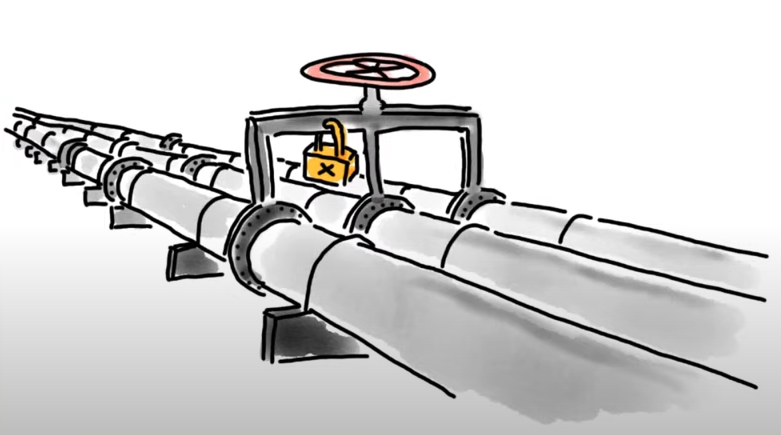
\includegraphics[scale=.43]{./assets/coupling.png}

    \textit{Is this one or three pipelines?}
  \end{center}
\end{frame}







\subsection{How to test microservices?}
\begin{frame}{Mocks}
  \begin{itemize}
    \item Mocking
  \end{itemize}
\end{frame}


\begin{frame}{Problem Statement}
  When organizations grow and so do the number of services
  \begin{itemize}
    \item How can we know, that the \textbf{whole} system works, when I publish changes?
    \item How can I avoid dependency on E2E tests for deployment and still be confident?
    \begin{itemize}
      \item Testing microservices in isolation is not enough
    \end{itemize}
  \end{itemize}
\end{frame}

\begin{frame}{Many hops...}
  \begin{itemize}
    \item Show here what it would mean for us to have pure e2e tests
  \end{itemize}
\end{frame}

\begin{frame}{Problems}
  \begin{itemize}
    [<+->]
    \item Local changes, even if tested, do not assure that the system as whole is working
    \item Loosely coupled architecture but tightly coupled teams. Such systems are - no matter the architecture - still monolithic from a CD perspective
  \end{itemize}
\end{frame}

\begin{frame}{Embedded Animation}
  \animategraphics[loop,controls,scale=.2]{2}{./assets/error-propagation/errProp-}{0}{6}
\end{frame}
